\documentclass[14pt,a4paper]{extarticle}
%\documentclass[12pt,a4paper]{article}

\usepackage[utf8]{inputenc}
\usepackage[ukrainian]{babel}


\usepackage{amssymb}
\usepackage{physics}


\usepackage[active]{srcltx}
\usepackage[final]{pdfpages}

\usepackage[hidelinks]{hyperref}

\usepackage{verbatim}
%%%%%%%%%%%%%%%%%%%%%%%%%%%%%%%%%%%%%%%%%%%%%%%%%%%%%%%%%%%%%%%%%%
%\pagestyle{empty}                     %нумерацiя сторiнок i т.д.
\pagestyle{headings}                   %нумерацiя сторiнок вгорi зправа i т.д.
%\renewcommand{\baselinestretch}{1.5}   %мiжстрiчковий інтервал
%\parindent=7.5mm                      %абзацний відступ
 \righthyphenmin=2                     %перенос 2 останніх букв
 \pagenumbering{arabic}
 \tolerance=400
 \mathsurround=2pt
 \hfuzz=1.5pt
%%%%%%%%%%%%%%%%%%%%%%%%%%%%%%%%%%%%%%%%%%%%%%%%%%%%%%%%%%%%%%%%%%
 \hoffset=-0.5cm        %+2.5cm -- вiдступ вiд лiвого краю
 \voffset=-1.5cm        %+2.5cm -- вiдступ зверху
 \oddsidemargin=0.1cm   %ліве поле
 \topmargin=0.1cm       %верхнє поле
 \headheight=0.5cm      %висота верхнього колонтитулу
 \footskip=1cm          %висота нижнього колонтитулу
 \headsep=0.3cm         %відступ від колонт. до тексту
 \textwidth=17cm        %ширина сторінки
 \textheight=25.5cm     %висота сторінки
%%%%%%%%%%%%%%%%%%%%%%%%%%%%%%%%%%%%%%%%%%%%%%%%%%%%%%%%%%%%%%%%%%
 \newcounter{e}
 \setcounter{e}{0}
 \newcommand{\n}{\refstepcounter{e} (\arabic{e})}
 
 \newcounter{pic}
 \setcounter{pic}{0}
 \newcommand{\pic}[1]{\refstepcounter{pic} \vspace{-0.3cm}\textit{Picture \arabic{pic}\label{#1}.}}
 
 \newcounter{tabl}
 \setcounter{tabl}{0}
 \newcommand{\tabl}[1]{\refstepcounter{tabl} \vspace{-0.3cm}\textit{Table \arabic{tabl}\label{#1}.}}
 
 \newcounter{dod}
 \setcounter{dod}{0}
 \newcommand{\dod}[1]{\refstepcounter{dod} \textit{Appendix \arabic{dod}\label{#1}.}}
 
% \newcounter{defn}
 %\setcounter{defn}{0}
 %\newcommand{\defn}[1]{\refstepcounter{defn} %\textbf{Означення \arabic{defn}\label{#1}.}}
 
 %\newcounter{theorem}
 %\setcounter{theorem}{0}
 %\newcommand{\theorem}[1]{\refstepcounter{theorem} %\textbf{Теорема \arabic{theorem}\label{#1}.}}
 \newtheorem{theorem}{Theorem}[section]
 \newtheorem{defn}[theorem]{Definition}
 \newtheorem{lemma}[theorem]{Lemma}
 
 \newcommand{\proof}{\textit{Proof. \space}}
% \setcounter{page}{1}
% \setcounter{section}{1}

\numberwithin{equation}{section}
\numberwithin{figure}{section}
%%%%%%%%%%%%%%%%%%%%%%%%%%%%%%%%%%%%%%%%%%%%%%%%%%%%%%%%%%%%%%%%%%
 \newcounter{stali}
 \setcounter{stali}{0}
 \newcommand{\s}{\refstepcounter{stali} \arabic{stali}}

 \newcommand{\st}{C_{\s}}
 \newcommand{\stl}[1]{C_{\s \label{#1}}}

 \newcommand{\cd}{{} $$ \vspace{-0.3cm} $$ {}}
 
 \newcommand{\nb}[2]{\righthyphenmin=#2 #1 \righthyphenmin=2}

%%%%%%%%%%%%%%%%%%%%%%%%%%%%%%%%%%%%%%%%%%%%%%%%%%%%%%%%%%%%%%%%%%
 
 \newcommand{\tabboxl}[2]{\parbox{#1}{\vspace{0.1cm} #2 \vspace{0.1cm} }}
 
 
 \newcommand{\tabboxr}[2]{\parbox{#1}{\vspace{-0.3cm}
 		\begin{flushright} #2 \end{flushright} \vspace{-0.3cm} }}
 
 \newcommand{\tabboxc}[2]{\parbox{#1}{\vspace{-0.3cm}
 		\begin{center} #2 \end{center} \vspace{-0.3cm} }}

 \newcommand{\liml}{\lim\limits}
 \newcommand{\suml}{\sum\limits}
 \newcommand{\intl}{\int\limits}
 
 \newcommand{\inttwopi}{\intl_{0}^{2\pi}}
 
 
 %%%%%%%%%%%%%%%%%%%%%%%%%%%%%%%%%%%%%%%%%%%%%%%%%%%%%%%%%%%%%%%%%%
 % bibliography
 %\usepackage[
 %backend=biber,
 %style=numeric,
 %sorting=none
 %]{biblatex}
 %\addbibresource{resources/bibliography.bibtex}
 %%%%%%%%%%%%%%%%%%%%%%%%%%%%%%%%%%%%%%%%%%%%%%%%%%%%%%%%%%%%%%%%%%

 \begin{document}
	
 %\bibliographystyle{insrt}

 \thispagestyle{empty}

 \begin{center}
	\large
	Міністерство освіти і науки, молоді та спорту України \\
	Львівський національний університет імені Івана Франка \\
	Факультет прикладної математики та інформатики \\
	Кафедра обчислювальної математики
 \end{center}

 \vspace{45pt}

 \vfill

 \begin{center}
	{\Huge{Магістерська робота}}\\
	{\large на тему:}
 \end{center}

 \begin{center}\Large
	\textbf{\emph{"Атаки на системи виявлення об'єктів"}}
 \end{center}

 \vfill
 \vskip100pt

 \begin{flushleft}
	\hskip8cm 
	Виконав:
	\\ \hskip8cm 
	студент II курсу групи ПМпМ-22с
	\\ \hskip8cm
	напрямку підготовки (спеціальності)
	\\ \hskip8cm
	113 -- ``Прикладна математика''
	\\ \hskip8cm
	Бугрій Б.О.
 \end{flushleft}

 \begin{flushleft}
	\hskip8cm 
	Науковий керівник:
	\\ \hskip8cm
	доц. Музичук Ю.А.
 \end{flushleft}

 \vfill

 \begin{center}
	\large
	Львів - 2022
 \end{center}

 \newpage
 \thispagestyle{empty}
 \renewcommand*\contentsname{Contents}
 \tableofcontents

\newpage
thispagestyle{empty}
\addcontentsline{toc}{section}{Abstract}
\section*{Abstract}
\begin{center}\end{center}

\begin{comment}
    Abstract:

Summary: The abstract provides a concise summary of the entire paper, including the purpose, methods, results, and conclusions. It is usually around 150-250 words long.
Purpose: It allows readers to quickly understand the essence of the research and decide if the paper is relevant to their interests or worth reading in full.
Stand-alone section: The abstract is a stand-alone section that can be read and understood independently of the rest of the paper. It is often used in literature searches, bibliographic databases, and conference proceedings.
Structure: The abstract generally follows a structure that covers the background, objectives, methods, results, and conclusions without going into too much detail.
\end{comment}

 \newpage
 \thispagestyle{empty}
 \addcontentsline{toc}{section}{Introduction}
 \section*{Introduction}
 \begin{center}\end{center}

In recent decades, thanks to smart artificial intelligence systems, humanity has made significant progress in various areas of everyday life. Notable examples include cars that can navigate difficult routes without human intervention, medical software that accurately diagnoses patients based on detailed information and test results, speech recognition and replication applications, and many others.

AI has had a significant impact on various industries, such as logistics, medicine, security, entertainment, and more. Computer Vision is one of the most common areas where AI is applied today. It focuses on using algorithms to solve complex problems based on visual data such as images and videos. Numerous algorithms and approaches have been developed to address this problem, including Convolutional Neural Networks (CNNs) \cite{overview}.

A significant part of these breakthroughs is due to the rapid development of Deep Neural Networks, which, compared to other machine learning algorithms, are able to show impressive results when powered by large data sets, sometimes even surpassing humans. They have been successful in detecting complex objects and shapes, and have demonstrated high performance in many applications. However, despite such capabilities, they sometimes face challenges when it comes to tasks such as recognizing road signs or counting the number of people in an image \cite{od-overview}.

People often trust their lives to systems, powered by machine learning. So it is crucial to be able to rely on predictions and decisions made by the system. Such mission-critical AI systems should maintain several properties to ensure their effectiveness, reliability, and overall performance. Along with confidentiality, scalability, adaptability, usability and transparency, a very important indicators of a good ML system are accuracy and robustness. A mission-critical AI system must deliver accurate and precise results, as its outputs can have a significant impact on decision-making. Ensuring accuracy requires proper training and validation of AI models on relevant and diverse datasets. A robust AI system must be able to handle unexpected inputs or situations without failing or producing incorrect results. Robustness is particularly important for mission-critical systems as they need to maintain reliable performance even in the face of unforeseen challenges or malicious actions.

If we start talking about robustness in more detail, we will be able to see various threats which can occur at different stages of AI development, from the early stages, when we even don't know which algorithm to choose to approach the selected problem, to model deployment into the real world. Our goal is to go through the process taking the attackers' point of view, perform and evaluate diverse attacks on the machine learning system.

For the experiments, we have chosen the object detection domain. Overall, the field of computer vision and object detection is rapidly evolving, and there is a continuous need for research and development to improve its performance and overcome its challenges. 

....

The mission-critical system we are going to build and attack is inspired by the ongoing war in Ukraine. We are going to build an enemy vehicle detection system, which should detect suspicious activity on the battlefield based on satellite images using state-of-the-art machine learning models. Then we are going to try to compromise it using different technics and evaluate the impact of the attacks.


Object detection has many applications, from autonomous vehicles to video surveillance and security. Another example of mission-critical object detection system is military vehicles detection on images taken by satellites or unmanned aerial vehicles. It can bring significant advantages on the battlefield, helping to quickly identify quantity and location of enemy forces. On the other hand, if the system’s integrity is violated, it might cause unwanted consequences. Therefore, there is a need to study its security and to be aware of possible threats.

We can solve this problem conveniently using Deep Neural Networks. Since the domain requires high accuracy and real-time performance, we use YOLOv5 [1] model as a core of our system. 

TODO add some images to this section. 


\begin{comment}
\end{comment}

\newpage
\thispagestyle{empty}
\section{Definition of the problem}

\begin{comment}
Statement of object detection

General statement of the adversarial attack

Various attack settings

- train time (poisoning)
   -(partial) access to the training data
   -
   -
   -access to the whole training process

- inference time (evasion)
   - evasion
\end{comment}

\subsection{Computer Vision tasks}
To understand what is object detection, let us consider the definitions of the following Computer Vision tasks:
\begin{itemize}
    \item \textbf{Object classification}, or multiclass classification is a problem in which the image consists of one main object and, usually, a background. The object belongs to one of two or more predefined classes. The model, given the input image, should return a class of the object from the image.
    
    \item \textbf{Object localization} is the task that aims to locate the target object within the image or video. There might be multiple instances of the object or even different classes of objects on the same image. The model, given the input image, should return the location of objects on the image in the specified formats, like coordinates of the center of the object or somehow defined area which contains the targets.
    
    \item \textbf{Object detection} has a goal of not only finding objects from a chosen set of classes on the image but also figuring out what these objects are. The model, given the input image, should return the location and class label of every specific object from the subject area.
\end{itemize}

So, as follows from the above descriptions, an object detection problem is a combination of object classification and object localization. It has its own challenges, which have to be addressed. For example, on one image there might be multiple objects of different shapes and sizes, viewed from angles, etc. This problem is also costly in terms of computational resources it requires since usually, we should use complex ML algorithms with a lot of parameters.

\subsection{Object detection model}

Let $\mathbb{X} := \{(r, g, b)^{n \times m} : r \in \mathbb{N}_0, r < 256,  g \in \mathbb{N}_0, g < 256, b \in \mathbb{N}_0, b < 256, \}$ be a set of images in the RGB format. Also, let's define $\mathbb{Y}:=\{(c, a_{1}, a_{2}, h, w)^k : c \in \mathbb{N}_0, c<C, a_1 \in [0, 1], a_2 \in [0, 1], h \in [0, 1], w \in [0, 1]\}$. For the given image $x \in \mathbb{X}$, there is $y \in \mathbb{Y}$ that describes all the objects from the area of interest on the image. In $y:=(c_i, a_{1i}, a_{2i}, h_i, w_i)^k_{i=0}$, the $i$-th component represents class $c_i$, position coordinates $(a_{1i}, a_{2i})$, height $h_i$ and width $w_i$ for one of $k$ objects, detected on the image $x$.

Let $M: \mathbb{X} \rightarrow \mathbb{Y}$ be an object detection model, meaning that it should localize and classify the set of objects on an image. Given an image $x \in \mathbb{X}$, it should produce prediction $y \in \mathbb{Y}$:
\begin{equation}
    M(x)=y
\end{equation}

Let $D = \{(x, y): x \in \mathbb{X}, y \in \mathbb{Y}\}$ be the set of initial data, images in RGB format, and corresponding labels for the object from the area of interest. We split it into three parts, such that:
\begin{equation}
    \begin{gathered}
        D = D_{train} \cup D_{val} \cup D_{test} \\
        D_{train} \cap D_{val} = \O\\
        D_{train} \cap D_{test} = \O\\
        D_{val} \cap D_{test} = \O\\
    \end{gathered}
\end{equation}
where $D_{train}$ -- training set, $D_{val}$ --  validation set, $D_{test}$ -- test set.

Let $\mathbf{V}(M, D_val) \in [0, 1]$ be a defined performance metric, which shows how good our model can predict TODO  

Let's define $\mathbf{T}$ as a training process, a sequence of actions to train the machine learning model on the specific dataset $D$, including weights optimization and hyperparameters tuning. If we say that $M_{0}$ is a model with defined architecture before training, and $M$ -- trained model, then:
\begin{equation}
    \mathbf{T}(M_{0}, D_{train}) = M  
\end{equation}
Our goal is to find $\mathbf{T}$ such that the final model $M$ satisfies certain performance metrics measured on $(x, y) \in D_{val}$. 

        
\subsection{Military vehicles detection}
\subsubsection{Advantages for military operations}
From a battlefield perspective, systems capable of detecting military vehicles in satellite images can provide critical advantages that directly impact the effectiveness of military operations. The benefits it offers are focused on strategic and tactical decision-making. The military vehicle detection system (MVD system) can efficiently process vast amounts of satellite imagery data, enabling them to analyze large geographical areas and detect military vehicles over extensive regions, which would be challenging and time-consuming with manual methods.

Real-time or near-real-time analysis of satellite imagery allows commanders to have an up-to-date understanding of enemy movements and positions, which is crucial for making informed decisions on the battlefield. The military vehicle detection systems enable commanders to make quick decisions in response to changing conditions, potentially giving them an advantage in battle. With accurate information on the composition and distribution of enemy forces, resources such as troops, vehicles, and air support, can be better allocated to counter threats effectively and optimize the strategies.

By continuously monitoring satellite images, we can identify potential threats, such as enemy build-ups, movements, or logistic activities, early on. This early warning capability allows us to take proactive measures to counter emerging threats. Also, the ability to detect and classify different types of military vehicles can help  identify high-value targets and prioritize their engagement, maximizing the effectiveness of the attacks and minimizing collateral damage.

Using MVD systems we can achieve enhanced reconnaissance and surveillance. The integration of satellite-based military vehicle detection with other intelligence sources, such as aerial reconnaissance and ground-based sensors, provides a more comprehensive picture of the battlefield, enabling more effective planning and execution of military operations.

In summary, systems that can detect military vehicles in satellite images provide a range of benefits from a battlefield perspective. By offering improved situational awareness, rapid decision-making, better resource allocation, and enhanced reconnaissance capabilities, these systems can significantly impact the effectiveness of military operations and contribute to achieving strategic and tactical objectives.







\subsubsection{Dataset generation}
\begin{comment}
    We would like to identify the positions of objects in an image, and to know what the object class is. So, having an image, we want to find the set of labels (object’s class, coordinates of object’s center on the image, width and height of an object) that represent position of each vehicle on the image.    
\end{comment}

Every model requires data ...

No existing dataset that suits our domain.
Examples ...

That's why we decided to simulate our task on the generated dataset. We are going to take civil satellite images and then combine them with images of military vehicles to generate the set of data $D$. We use two sets of images: backgrounds and objects from the area of interest.

At first, as a background set, we use data from the DOTA TODO \ref{dota} dataset. The DOTA images are collected from the Google Earth, GF-2 and JL-1 satellite provided by the China Centre for Resources Satellite Data and Application, and aerial images provided by CycloMedia B.V. DOTA consists of RGB images and grayscale images. The RGB images are from Google Earth and CycloMedia, while the grayscale images are from the panchromatic band of GF-2 and JL-1 satellite images. All the images are stored in 'png' formats \ref{dota}. The dataset also contains labels for objects like cars, boats, swimming pools, football fields, and many others, but we are omitting these labels because we are not interested in detecting such objects.

\begin{center}
    \includegraphics[height=5cm]{images/satelites.png}
\end{center}


The second set of images should contain military vehicles of different classes. At this moment, we are going to distinguish three classes:
\begin{itemize}
    \item infantry fighting vehicles (IFV)
    \item multiple rockets launch systems (MLRS) 
    \item tanks
\end{itemize}
\begin{comment}
    artillery?
\end{comment}
We used different publicly available resources to gather images of representatives of these classes. Some examples are displayed in the picture \ref{}.

\begin{center}
    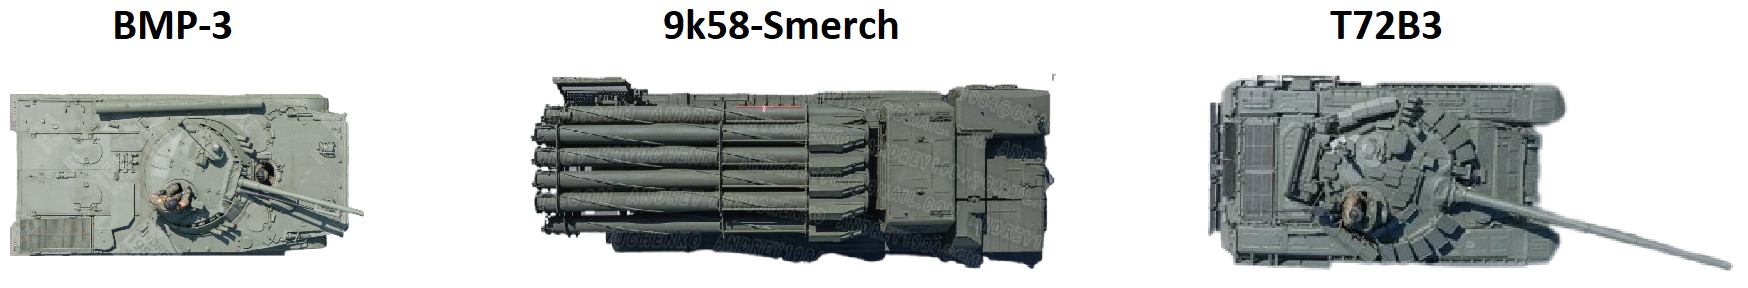
\includegraphics[height=5cm]{images/military-vehicles.png}
\end{center}


TODO generation process and sizes of sets



\newpage
    \subsection{Evaluation metrics}
        \subsubsection{Intersection over Union}
To be able to compare the performance of our models and tell how good they are at detecting objects on the images, we need to have a defined metric.
We are trying to predict the bounding box which contains the object. But it is usually expected that the predicted and ground-truth boxes will not match. So usual metrics, like accuracy, can't be applied, since it is designed for a completely different type of problem.

%Let us imagine two bounding boxes, as on the picture below. 
It is hard to determine, which prediction is better. It is logical to consider the area of the predicted bounding box which is covering the ground-truth region. But what if it just covers most of the image? Therefore another quantitative measure is used to compare true data with the results of the predictions, called \textit{IoU}, \textit{Intersection over Union}, which is computed by the following formula:
\begin{equation}
    IoU = \frac{B_1 \cap B_2}{B_1 \cup B_2}
\end{equation}
Basically, it is the Jaccard index of the two sets.
It is obvious that values of this metric differ from 0 (no overlapping area at all) to 1 (exact match). So, the greater the region of overlap, the greater the IoU. You can see the visual representation of the parts of this formula in the picture below.

\begin{center}
    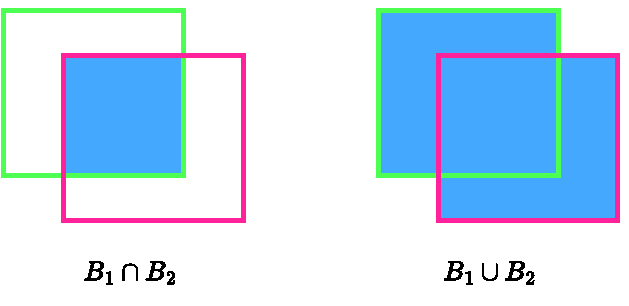
\includegraphics[width=10cm]{images/iou.pdf}
\end{center}

Now we are able to calculate the average of these metrics over the batch of data or the whole training set to easily measure models' performance. This may be  appropriate if we are solely interested in the quality of the predicted bounding boxes. But there is a metric that can provide a better understanding of a model's overall performance in object detection tasks. We are going to discuss it in the following chapter.

        
        \subsubsection{Average Precision}
Mean average precision is a popular and comprehensive metric when it comes to the evaluation of object detection model \ref{map}.
To define what the \textit{average precision} and the \textit{mean average precision} are, we first should understand what is the confusion matrix and how it is calculated.

In binary classification, the \textit{confusion matrix} is a table that evaluates all the outcomes of the classification. Taking into account that there are two states, the object actually belongs to the class or not belongs to it, and the same two possible outcomes of prediction, having some set of data we can divide all the predictions made into four groups. They are usually displayed as a table:

\begin{center}
    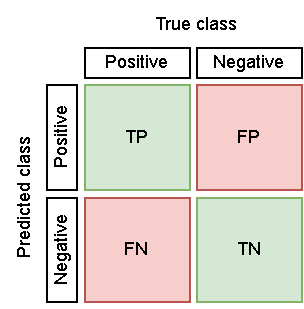
\includegraphics[width=5cm]{images/confusion-matrix.pdf}
\end{center}

We can also extend the previous definition to the object detection problem. At first, some IoU threshold is defined, to understand, if the object was detected or not. For example, if we choose an IoU threshold equal to 0.5, we say that the object was detected in case the IoU of the predicted bounding box and ground truth is greater or equal to 0.5. Then for each class, we are able to calculate the following:
\begin{itemize}
    \item \textbf{True positives} -- the object was on the image, and it was detected by a model.
    \item \textbf{False positives} -- the was no object on an image, but the model detected that it was there
    \item \textbf{False negatives} -- the object was on the image, but the model detected no object there.  
\end{itemize}
True negatives are not defined for the object detection problem, because it is not possible to numerically express the number of objects, that were not on the image and were not detected.

Now, based on TP, FP and FN we are able to calculate other metrics, such as Precision and Recall. They are calculated for each class separately. They are particularly useful in the context of imbalanced datasets or imbalanced model predictions. These metrics help to provide insights into the effectiveness of a model in terms of its ability to correctly identify true positives and true negatives while minimizing false positives and false negatives.

\textit{Precision} is the proportion of true positives (relevant instances correctly identified by the model) among the total number of instances predicted as positive by the model. It measures the model's ability to accurately identify only the relevant instances, minimizing false positives.

TODO

Precision: tells us how precise our model is i.e. out of total detected say cats, how many were actual cats. Hence, it is the ratio between the true positive and the total number of cat predictions (equivalently the sum of true positive and false positive) made by the model as shown below.
Recall: Tells us how good the model is at recalling classes from images i.e. out of total cats in the input image how many was the model able to detect. Hence, it is the ratio between the true positive and the total number of ground truth cats (equivalently the sum of true positive and false negative) made by the model as shown below.

\begin{equation}
    \begin{gathered}
        \text { Precision }=\frac{\text { Correct Predictions }}{\text { Total Predictions }}=\frac{T P}{T P+F P} \\
        \text { Recall }=\frac{\text { Correct Predictions }}{\text { Total Objects }}=\frac{T P}{T P+F N}
    \end{gathered}
\end{equation}

TODO Precision recall curve

\begin{equation}
    \mathrm{AP}=\int_{r=0}^1 p(r) d r
\end{equation}


We use the mean average precision (mAP) to evaluate the performance of our object detection model. It is calculated by the following formula:
\begin{equation}
    m A P=\frac{1}{k} \sum_i^k A P_i 
\end{equation}

Here k – number of classes, AP – average precisions. AP is calculated with the help of several other metrics such as IoU (intersection over union), confusion matrix (TP, FP, FN), precision and recall [4]. It equals an area under precision-recall curve calculated for specified IoU threshold.



\newpage
\thispagestyle{empty}
\section{Object detection}
\subsection{Multistage vs Single Stage}
\subsection{YOLO}
\subsubsection{Versions overview}
TODO add refs
        
YOLOv5, or "You Only Look Once version 5", is an object detection model that builds upon the previous iterations of the YOLO series. YOLO is a popular deep learning algorithm known for its speed and accuracy in detecting objects in images and videos. The history of YOLO can be divided into different versions, leading up to YOLOv5.

YOLOv1 was introduced by Joseph Redmon and Ali Farhadi in their 2016 paper titled "You Only Look Once: Unified, Real-Time Object Detection". YOLOv1 was a breakthrough in object detection as it provided real-time performance with reasonable accuracy. The primary innovation of YOLO was to treat object detection as a single regression problem, predicting bounding boxes and class probabilities directly from the image.

Also known as YOLO9000, YOLOv2 was introduced in a paper titled "YOLO9000: Better, Faster, Stronger" by Joseph Redmon and Ali Farhadi. YOLOv2 improved upon the original version by using anchor boxes, batch normalization, and higher-resolution input images. These changes resulted in better accuracy while maintaining the fast detection speed of the original YOLO.

Joseph Redmon and Ali Farhadi further improved YOLO with the release of YOLOv3, detailed in the paper "YOLOv3: An Incremental Improvement". YOLOv3 introduced multi-scale predictions using three different scales with varying sizes of anchor boxes. This allowed the model to better detect objects of different sizes in images. It also adopted the Darknet-53 backbone for feature extraction, significantly improving the model's accuracy while maintaining a fast inference time.

Joseph Redmon discontinued his work on the YOLO project; however, researchers Alexey Bochkovskiy, Chien-Yao Wang, and Hong-Yuan Mark Liao continued to develop the model. In April 2020, they published a paper titled "YOLOv4: Optimal Speed and Accuracy of Object Detection", which introduced YOLOv4. The new model integrated several state-of-the-art techniques, such as the CSPNet and PANet, and used the EfficientDet backbone. These changes resulted in significant improvements in both speed and accuracy.

YOLOv5 was released in May 2020 by Glenn Jocher, the founder of Ultralytics. It is not an official continuation of the original YOLO series, but it builds upon the work of previous versions. YOLOv5 uses custom neural network architectures, from a smaller one, called YOLOv5n, to the most advanced YOLOv5x, which is faster and more accurate than YOLOv4. It also includes enhancements such as automatic model scaling, improved data augmentation, and using PyTorch for easier implementation and deployment.
        \subsubsection{Layers}
        \subsubsection{Architecture}
        Backbone, neck, head

        \subsubsection{Anchor boxes}
        \subsection{Loss function}
        
        \subsubsection{Non-Maximum Suppression}

\newpage
\thispagestyle{empty}
\section{Adversarial attacks}
\subsection{Overview}
In machine learning, any malicious action performed with a machine learning model by a third party, in order to benefit from it in a ``bad'' way can be called \textit{adversarial attack}.
There are three main types of adversarial attacks:
TODO
\begin{itemize}
    \item Evasion (impacts model performance by changing the input)
    \item Poisoning (impacts model performance by changing the model)
    \item Extraction (does not impact model, extracts sensitive information) (data extraction vs model stealing)
\end{itemize}

    
    
    \subsection{Attack settings}
    white box
    black box

\subsection{Data poisoning}
\subsubsection{Definition of the problem}
\begin{comment}
    backdoor vs lowering accuracy by missing labels
\end{comment}

The idea of data poisoning is to modify the $D_{train}$ in order to lower the performance of the machine learning model $M$. We need to find transformation $p$ on the training image and its label:
\begin{equation}
    \label{poisonin}
    p(x, y) = (x', y')
\end{equation}
Then we construct $D_{poisoned}=\{p(x, y) : (x, y) \in D_{train}\}$ -- a set of poisoned data. We assume that the attacker is able to modify only a small part of the data, so $D'_{train} = D_{clean} \cup D_{poisoned}$, where $D_{clean} \subset D_{train}$, and $n(D_{poisoned})$ is significantly smaller than $n(D_{clean})$. Equation \ref{posoned-model} defines the model, trained on poisoned data. We call it \textit{poisoned model}.

\begin{equation}
    \label{poisoned-model}
    \mathbf{T}(M_{0}, D'_{train}) = M'
\end{equation}

Define validation set



TWO CASES simple poisoning vs backdoor attack

Find p such that the performance of M' $\approx$ performance of M on Dval, but performance of M' $\ll$ performance of M on D'val 

TODO poisoned training

\subsubsection{Backdoor attacks}

    \subsection{Main algorithms}
    \subsection{Real-world attacks?}
    \subsection{Defence strategies?}

\newpage
\thispagestyle{empty}
\section{Experiments and evaluation}
    \subsection{Model for enemies detection}
        \subsubsection{Simple settings}
        \subsubsection{Advanced model}
        \subsubsection{Performance metrics}

    \subsection{Attacks}
    \subsubsection{Missing/incorrect labels}
    \subsubsection{Data poisoning}
\begin{center}
    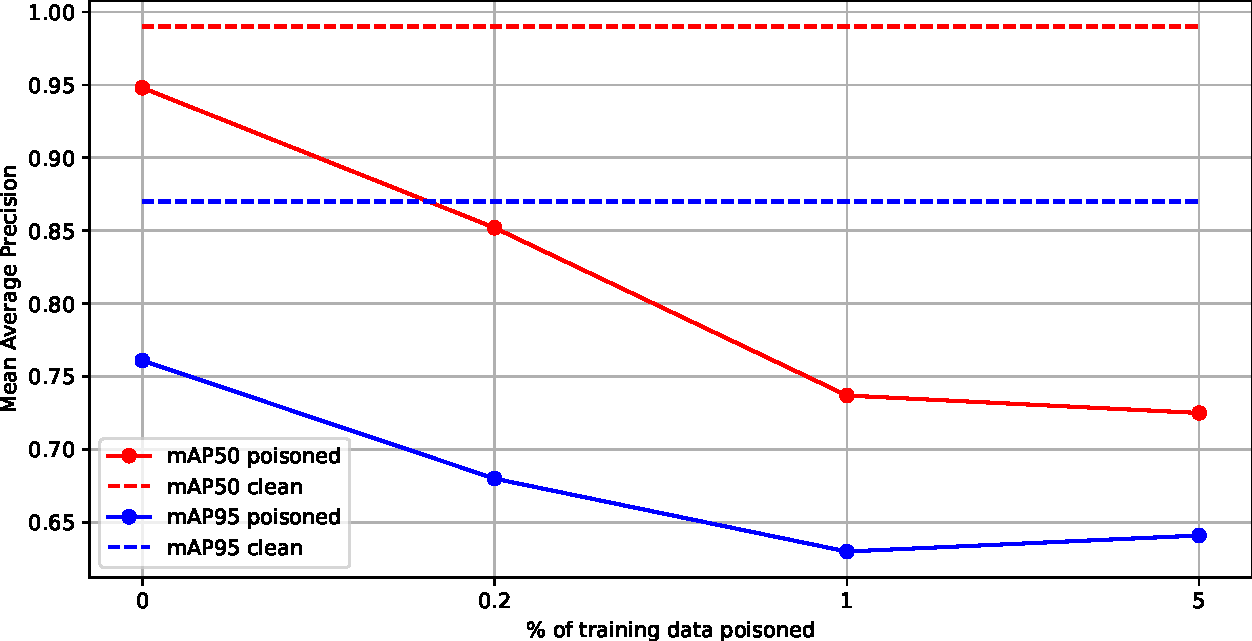
\includegraphics[width=14cm]{images/robustness.pdf}
\end{center}
\begin{comment}
    \subsection{Model under attack}
        \subsubsection{White box}
        \subsubsection{Performance metrics}
    \subsection{???}
        \subsubsection{Transferability from classification models}
        \subsubsection{Data from different distributions}
\end{comment}
\newpage
\thispagestyle{empty}
\section{Conclusions}


\newpage
\thispagestyle{empty}
\addcontentsline{toc}{section}{Appendix}
\section*{Appendix}
\dod{dod-1}
\begin{center}
    
\end{center}
 
\newpage
\thispagestyle{empty}
\addcontentsline{toc}{section}{Bibliography}
\begin{thebibliography}{99}

    \bibitem[10]{map}
    https://towardsdatascience.com/what-is-average-precision-in-object-detection-localization-algorithms-and-how-to-calculate-it-3f330efe697b


    \bibitem[1]{overview}
    Z. Zou, Z. Shi, Y. Guo, J. Ye /
    Object Detection in 20 Years: A Survey. :
    arXiv preprint arXiv:1905.05055 (2019)

    \bibitem[2]{od-overview}
    \textit{Xiaoke Shen} /
    A survey of Object Classification and Detection based on 2D/3D data :
    arXiv preprint arXiv:1905.12683 (2022)

    \bibitem[3]{dog-cat}
    \textit{Great Learning Team} /
    Real-Time Object Detection Using TensorFlow :
    \href{https://www.mygreatlearning.com/blog/object-detection-using-tensorflow/}{mygreatlearning.com}

    \bibitem[4]{my-work-1}
    \textit{Богдан Бугрій} /
    Атаки на глибокі нейронні мережі :
    Львів (2020)

    \bibitem[5]{my-work-2}
    \textit{Богдан Бугрій} /
    Розробка алгоритмів захисту від атак на глибокі нейронні мережі :
    Львів (2021)

    \bibitem[6]{kernel}
    \textit{Axel Thevenot} /
    A visual and mathematical explanation of the 2D convolution layer and its arguments :
    \href{https://towardsdatascience.com/conv2d-to-finally-understand-what-happens-in-the-forward-pass-1bbaafb0b148}{towardsdatascience.com}

    \bibitem[7]{multi-output}    
    \textit{Kaushal Shah} /
    Building Multi Output Cnn With Keras :
    \href{https://kaushal28.github.io/Building-Multi-Output-CNN-with-Keras}{kaushal28.github.io}

    \bibitem[8]{pooling}
    \textit{Jason Brownlee} /
    A Gentle Introduction to Pooling Layers for Convolutional Neural Networks :
    \href{https://machinelearningmastery.com/pooling-layers-for-convolutional-neural-networks}{machinelearningmastery.com}
 

    \bibitem[9]{normalization}
    \textit{Martin Riva} /
    Batch Normalization in Convolutional Neural Networks :
    \href{https://www.baeldung.com/cs/batch-normalization-cnn}{baeldung.com}

    \bibitem[10]{textures}
    \textit{Raitis G.} /
    Battle City tanks repository :
    \href{https://github.com/raitisg/battle-city-tanks}{github.com}

    \bibitem[11]{gradient-descent}
    \textit{Sebastian Ruder} /
    An overview of gradient descent optimization algorithms :
    arXiv preprint arXiv:1609.04747 (2017)

    \bibitem[12]{activations}
    \textit{Johannes Lederer} /
    Activation Functions in Artificial Neural Networks: A Systematic Overview :
    arXiv preprint arXiv:2101.09957 (2021)

    \bibitem[13]{adversarial}
    \textit{Christian Szegedy, Wojciech Zaremba, Ilya Sutskever, Joan Bruna, Dumitru Erhan, Ian Goodfellow, Rob Fergus} /
    Intriguing properties of neural networks :
    arXiv preprint arXiv:1312.6199 (2014)

\end{thebibliography}

\end{document}
